
\chapter{绪论}
\echapter{Preface}

视觉在是人类的重要感官之一,也是人类获取信息效率最高的感官,是人类认识和理解外界的重要途经,计算机视觉也相应成为了人类社会工业界的重要支柱技术之一。随着深度学习的广泛应用,计算机视觉在近年有了蓬勃的发展,人体姿态估计(HPE, Human Pose Estimation)任务也被注入了新的活力,有了越来越多的科研成果。同时随着基于摄像头的计算机视觉解决方案的广泛铺开,人体姿态估计也逐渐贴合了越来越多的实际场景,在人机交互、游戏、虚拟现实、视频监控、运动分析、医疗辅助等领域有着广泛的应用,是计算机视觉领域的热门研究课题。本文基于单目摄像头的视频采集,利用深度神经网络,完成了视频序列中单人的人体姿态估计任务,并有效地利用提取出的动作制作了人体模型三维动画。



\section{应用背景与意义}


人体姿态估计在实际应用中,为视频监控、行为分析、自动驾驶、虚拟现实、人机交互(HCI, Humancomputer interaction)、医疗辅助、游戏、电影和动画等多种场景提供了丰富的人体几何和运动信息。
\begin{figure}[h!]
  \centering
  \subfloat[人体姿态估计辅助体育运动分析] {
      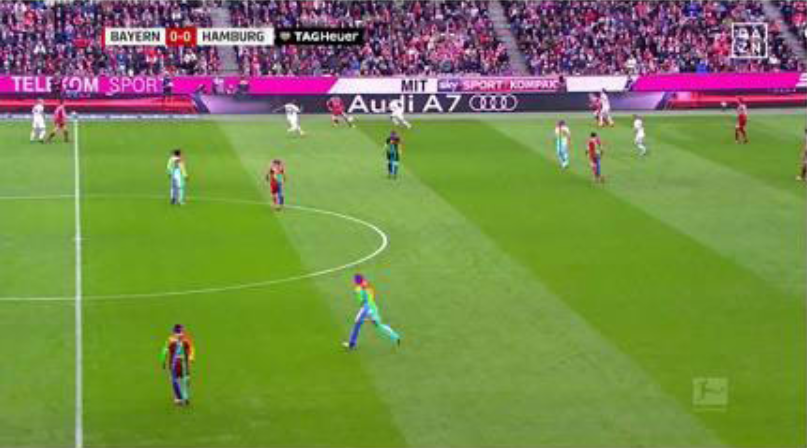
\includegraphics[width=6.67cm]{figures/1.png}
      \label{fig:f1}}
  \subfloat[基于人体姿态估计的体感游戏] {
      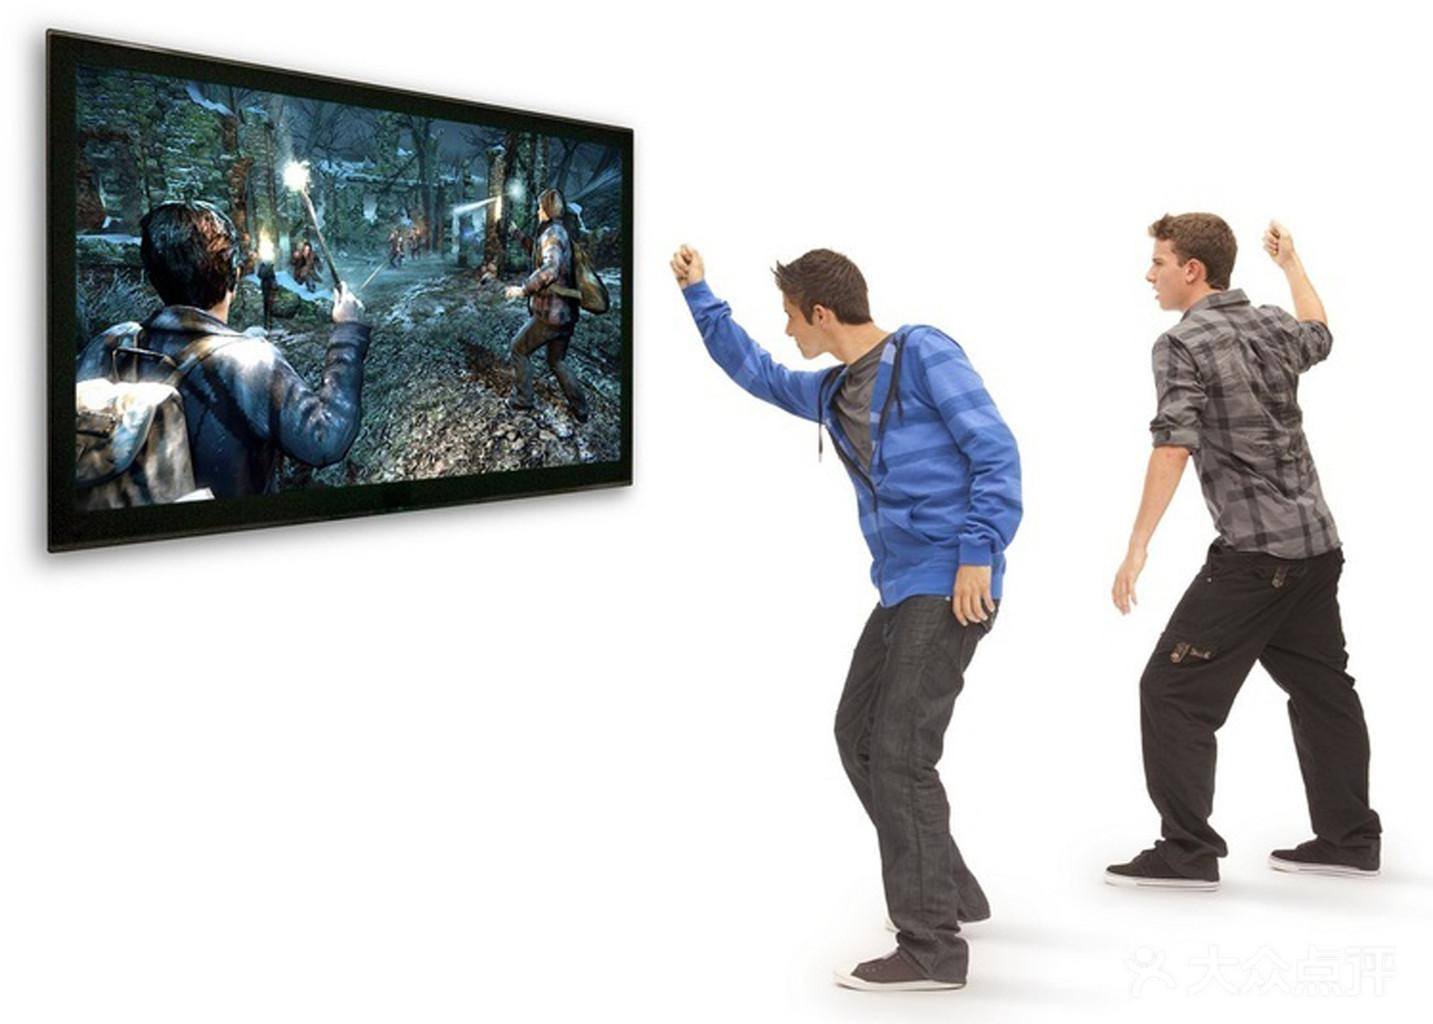
\includegraphics[width=6.67cm]{figures/2.png}
      \label{fig:f2}}
  \caption{人体姿态估计实际应用}
\end{figure}
例如在视频监控中,利用人体识别与人体姿态识别,可以实时监控楼宇、工地、社区等场所的高风险区域,发现攀高等危险行为时及时告警提醒,避免异常攀高导致安全事故;或对公共场所中人员突然奔跑或突然的人员聚集等情况进行检测和预判,助于安防疏导。在行为分析方面,如图\ref{fig:f1}所示,人体姿态识别可以辅助体育运动和训练中,对运动员或训练者的动作进行分析,分析其运动的习惯,辅助教练对不规范动作进行纠正等。在自动驾驶的研发中,需要对车辆行驶的路况进行分析和预测,此时需要对行人的朝向,姿态进行分析,进而预测可能的下一步行为,帮助车辆依此进行行驶决策。在人机交互中,如图\ref{fig:f2}所示,可以利用对人体动作的识别研发远程交互式体感游戏。

人体姿态识别在近年来成为了人类社会各类产业中辅助生产的重要技术之一,本文的工作则将人体姿态识别应用在了影视动画创作领域,利用对视频中人体动作的分析,自动化生成具有相应动作的三维角色动画。

动作捕捉(MoCap, Motion Caption)是记录运动并在数字角色模型上创建运动的过程。动作捕捉可用于各种应用场景,例如运动,医疗应用,人体工程学,娱乐和机器人技术,以及三维角色动画,预可视化以及虚拟电影制作。更为具体地,当动作捕捉应用于游戏开发和电影制作中时,则主要指记录演员动作,来制作动画等具有视觉效果的媒体内容。

\begin{figure}[h]
	\centering
	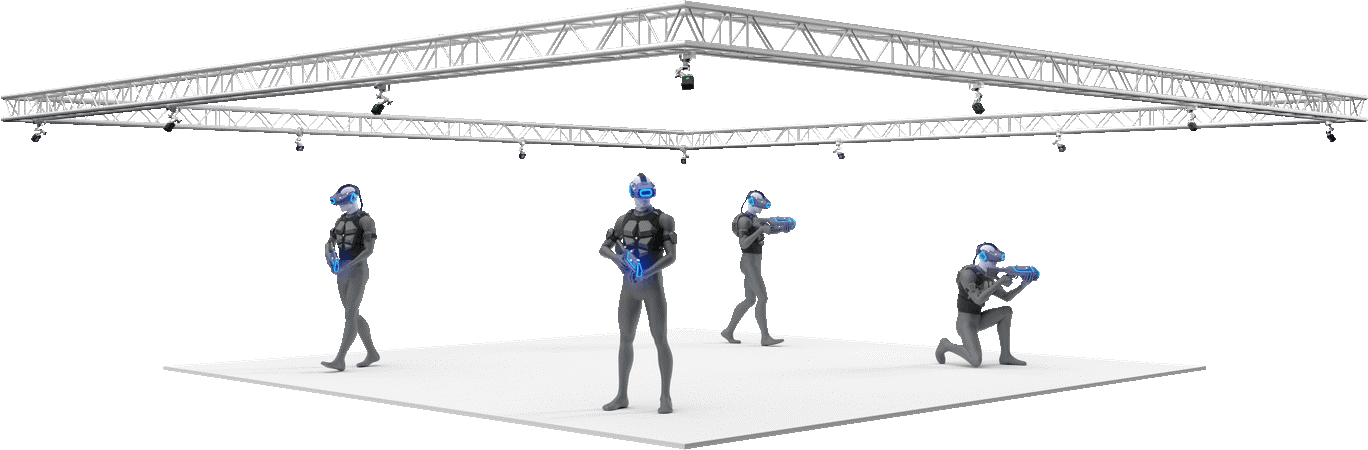
\includegraphics[scale=0.4]{figures/3.png}
	\caption{动作捕捉场地}
	\label{fig:f3}
\end{figure}

而这其中的主要动作捕捉技术主要依赖于硬件设备,从硬件设备的采集数据的原理上来说可以分为光学式、惯性式等。而除了一般动作捕捉系统中的穿戴式设备外、感应摄像头、符合光线要求的场地场所、相应软件以及基础的服务等对专业性的要求极高,价格不菲。根据相关调研报告,全球动作捕捉市场在2018年达到了1.632亿美元,并且预计到2026年,可以增长至2.617亿美元。同时预测复合年增长率在2019-2026年内为8.13%。

由于动作捕捉的价格昂贵,市场需求大,对动捕质量的要求随着动画产业的发展也在不断地增加。同时随着三维人体姿态估计的效果逐步提升,基于RGB摄像视频的动作捕捉成为了降低动画生成门槛的新的解决方案。



\section{课题主要任务}{}

人体姿态估计指在从图像或视频中,对任务目标的姿态进行识别和估计。

输入数据一般为采集的RGB图像或RGB-D图像,可以为单目单视角(Monocular)图像或使用多个摄像机针对相同的目标同一时刻的动作进行采集的多目多视角(Multi-view)图像,图像中可以包含一个人体目标或多个人体目标。

首先通过人体识别获得每个目标人体所在的区域或边框(bounding box),进一步通过热力图(heatmap)

对人体的各个关键点位置进行概览预测或直接回归出各关键点的坐标。可以通过对头部、颈部、髋部、膝盖等人体的重要关节点进行坐标预测来描述人体骨架,或通过估计出符合人体形状的蒙皮描述人体的姿态,例如图\ref{fig:f4}右侧蒙皮图像所示,SMPL模型(Skinned Multi-Person Linear (SMPL) Model),便利用具有10个维度的形状参数和描述24个关节点的姿态参数描述整个人体的蒙皮。

\begin{figure}[h]
	\centering
	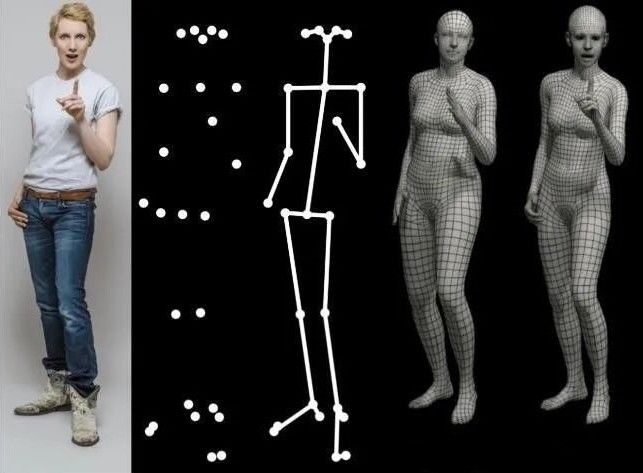
\includegraphics[scale=0.6]{figures/4.jpg}
	\caption{人体姿态描述模型}
	\label{fig:f4}
\end{figure}

此外,可以仅针对单帧图像进行估计,也可以在视频中,针对帧序列中的人体进行姿态序列的分析。在对帧序列进行姿态估计时,需要对同一个目标人物进行追踪,并利用时序模型来提取上下文信息,估计出准确连贯的姿态序列。

最为主要地,根据输出的数据维度,也即描述人体姿态关节点的坐标维度,可以划分为二维人体姿态估计与三维人体姿态估计两大部分。二维人体姿态估计的目标是定位图像中每个关键点的(x,y)坐标,而三维人体姿态估计的目标是推断三维空间中每个关键点的(x,y,z)坐标。

本文的工作主要集中在了对单目单人RGB视频中的目标进行姿态估计。基于此类数据的人体关节点坐标的恢复具有其独特的特征和挑战,其挑战主要在于三点:

其一,柔性体构型意味着复杂的相互依赖的关节和高自由度的肢体,这可能会导致出现自遮挡及其他罕见且复杂的姿态。

其二,是人体呈现的多样性,包括服装的多样及自身极为相似的部位。

其三,复杂的拍摄环境常导致前景的遮挡,加之多样的拍摄角度和画幅的不完整,导致目标与周围人的相似部位出现混淆。



\section{国内外研究现状}

\subsection{二维人体姿态估计}{}

早期的二维人体姿态估计融入了许多特征的构建,比如描述运动信息的梯度方向直方图(HOG, Histogram of Oriented Gradient)和小边特征(Edgelet)
等,但这些方法在实践中并不具备精确估计的能力。随着深度神经网络的发展,深度学习方法则更能够从元数据重提取出更充分的特征,产生了优异的结果,并在很大程度上超过了传统方法。基于方法分类的二维人体姿态估计任务如图\ref{fig:f5}。

\begin{figure}[h]
	\centering
	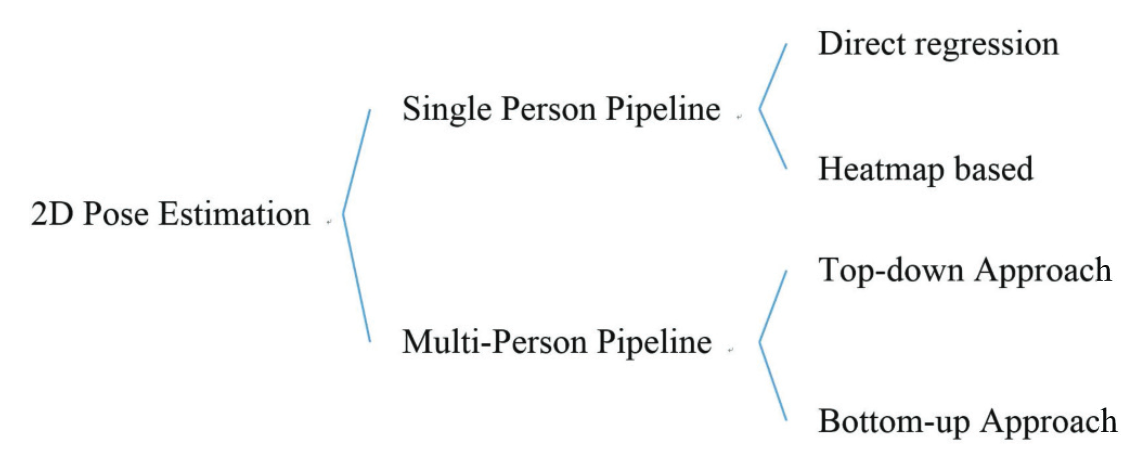
\includegraphics[scale=0.6]{figures/5.png}
	\caption{二维人体姿态估计分类}
	\label{fig:f5}
\end{figure}

单人姿态估计从预测关键点的方法上主要分为直接回归方法与热力图方法两类。前者利用输出特征映射直接回归关键点,如facebook于2018年搭建的DensePose。后者则首先生成热图(heatmap),用其中的像素值表示关键点在该位置存在的概率,并根据热图预测关键点,如2016年的Hourglass。

而多人姿态估计的整体思路主要分为两类。第一种为自顶向下的方法,指的是首先从全图的范围上进行人体检测,然后切入到每个目标人体的范围,进行单人关键点估计,如2016年提出的AlphaPose。自底向上的方法的第一步则是定位图像中的所有关节点,第二步是将关节点向上分组为人体,2016年提出利局部关联域(PAF, Part Affinity Field)方法进行关键点组装的OpenPose。

\subsection{三维人体姿态估计}{}
三维人体姿态估计相对于二维人体姿态估计具有更多难点,其一是单目图像及视频信息本身具有的歧义性,即一个二维的姿态投影可以对应多种三维的姿态。其二是需要利用昂贵的设备和严苛的环境条件进行三维姿态数据集的采集较为困难,故而对网络的泛化性要求也更为严格。

\begin{figure}[h]
	\centering
	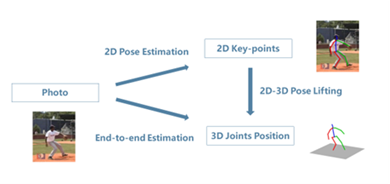
\includegraphics[scale=1]{figures/6.png}
	\caption{三维人体姿态估计两大思路}
	\label{fig:f6}
\end{figure}

如图\ref{fig:f6}所示,基于深度学习的三维人体姿态估计方法可主要分为两大思路。第一种思路为两步式,先从图像中提取出二维关节点坐标,再将其从二维提升到三维坐标,如Facebook AI于2018年提出的VideoPose三维模型。第二种思路为端到端式,从视频和图像中直接回归出三维坐标,如Li等于2014年利用卷积神经网络搭建的包括关节检测与坐标回归两支路模型。此外,还有工作选择融合式模型,在两步式的第二步估计过程中仍然融入源数据。

\subsection{视频动作捕捉}{}
无硬件设备需求的视频人体动作捕捉解决方案提供商在近几年,于国内外如雨后春笋般崛起并在持续地发展。

如国内云舶提供的对单人视频进行捕捉的小K动捕,对人物的脚-地接触进行了优化,使其接触稳定,无垂直的浮动。此外,美国DeepMotion也提供了包含单人动作捕捉以及人物追踪等多种视频解决方案。同时,Ridical也提供了粒度细至手指关节的实时视频动作捕捉API。

\begin{figure}[h]
	\centering
	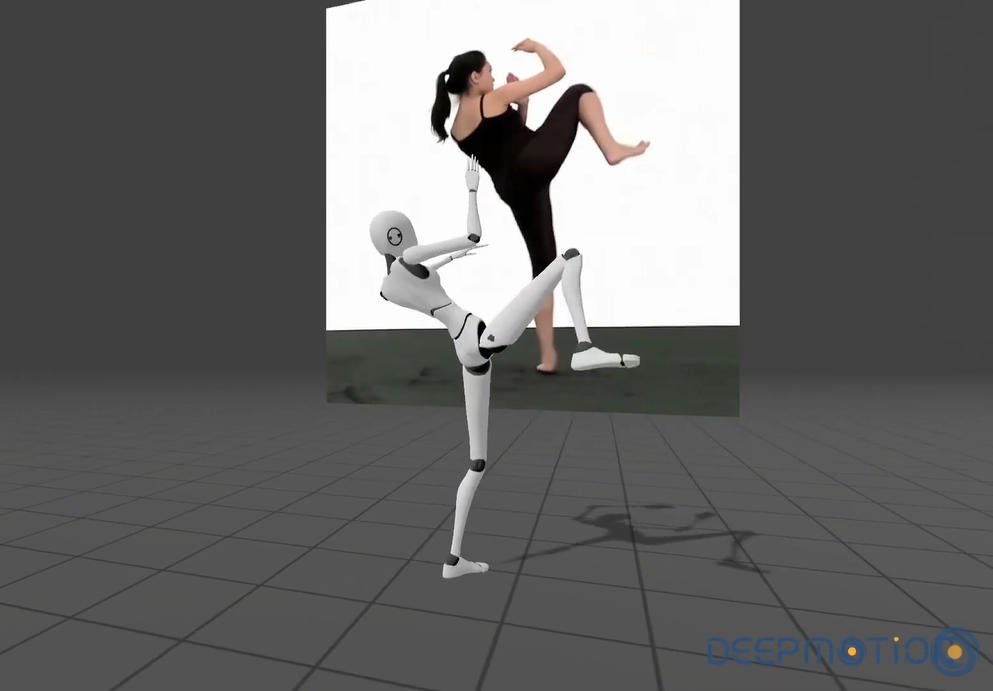
\includegraphics[scale=0.4]{figures/7.png}
	\caption{DeepMotion视频动作捕捉}
	\label{fig:f7}
\end{figure}



\section{本文主要工作内容}


\subsection{本文工作}{}
针对人体姿态估计任务,本文的工作主要聚焦到了基于深度神经网络模型,对日常场景中,单目RGB摄像头采集的单人动作视频进行姿态估计,并利用估计出的人物动作制作三维角色动画。整体流程首先输入单人视频,利用残差网络搭建二维关节点估计模型,并利用一维空洞卷积提取视频中的时序信息,将二维关节点坐标提升为三维坐标,最后将三维坐标转换为描述动作文件的人体骨架欧拉角,进行三维角色绑定。

\subsection{论文结构安排}{}
本文共包含六个章节,各章节的具体内容概括如下。

第一章:绪论。在绪论中,首先介绍了人体姿态估计课题的研究意义以及在各实际领域的应用价值,尤其是在动作捕捉领域,具有旷阔的市场和可期的前景。接着介绍了人体姿态估计的任务的具体目标及当前工作的研究现状。最后对本文的主要工作进行了简要的概括 ,并对本文的章节安排进行了介绍。

第二章:人体姿态识别相关基础。在第二章中,针对计算机视觉尤其是人体姿态估计中常用到的经典的深度学习模型及方法进行了介绍,包括卷积神经网络、残差网络等,它们构成了第三章及第四章模型的基础架构。同时介绍了人体姿态描述模型与动作捕捉相关设备与数据文件。

第三章:基于反卷积神经网络的二维人体姿态估计。本章重点说明了用于二维人体姿态估计的模型,一个相对于之前的Hourglass和CPN结构都更为简单明了的网络结构。模型利用热力图对人体关节进行二维坐标的预测,并在网络中利用反卷积进行上采样,用以得到高分辨率的特征图。

第四章:基于空洞卷积神经网络的三维人体姿态序列估计。本章首先针对三维人体姿态估计任务的主要问题进行了分析,并采用了二步提升法,同时利用卷积神经网络处理视频中的时序信息,进行三维人体姿态的估计。

第五章:视频动作捕捉动画生成。在本章中,利用第三章及第四章的网络模型所预测出的人体姿态,对人物角色模型进行动画生成。搭建了人体骨骼模型,将关节点坐标转换为了动作描述文件bvh所需的欧拉角。并在MotionBuilder软件中对人物模型进行了动作绑定,制作出了还原度极高且稳定的三维动画。

第六章:总结与展望。本章归纳和总结了本文针对人体姿态估计任务所做的工作,以及针对视频动作捕捉进行的工程搭建。对人体姿态估计的后续研究方向以及视频动作捕捉的未来进行了更深层次的探讨和展望。



